\documentclass[11pt]{article}
\usepackage{amsmath, amssymb, amsthm}
\usepackage[retainorgcmds]{IEEEtrantools}

\usepackage{marginnote}
\usepackage{endnotes}

\usepackage{tikz}
\usetikzlibrary{intersections}

\usepackage{fancyhdr}

%Listings stuff
\usepackage{listings}
\usepackage{lstautogobble}
\usepackage{color}

\definecolor{grey}{rgb}{0.5,0.5,0.5}
\lstset{
basicstyle={\small\ttfamily},
tabsize=3,
numbers=left,
numbersep=5pt,
numberstyle=\tiny\color{grey},
stepnumber=2,
breaklines=true
}

%Properly formatted differential 'd'
\newcommand{\ud}{\, \mathrm{d}}

%Format stuff
\pagestyle{fancy}
\headheight 35pt

%Header info
\chead{\Large \textbf{Vectors}}
\lhead{}
\rhead{}

\begin{document}
\section{Basics}
	Definition: A vector $\vec{x}$ is defined as a collection of $n$ ordered numbers $(x_1, x_2,\ldots ,x_n)$.
	
	Basic properties:
	\begin{itemize}
		\item $c(\vec{x} + \vec{y}) = c\vec{x} + c\vec{y}$
		\item $(\vec{x} + \vec{y}) + \vec{z} = \vec{x} + (\vec{y} + \vec{z})$
		\item $(a+b)\vec{x} = a\vec{x} + b\vec{x}$
	\end{itemize}
	
	Other concepts/terms:
	\begin{itemize}
		\item Zero vector: $\vec{0} = (0, 0,\ldots , 0) \text{ and } \vec{x} + \vec{0} = \vec{x} \ \forall \vec{x}$
		\item The \textbf{linear combination} of vectors $\vec{x_1}, \ldots , \vec{x_k} \text{ is } c_1\vec{x_1} + c_2\vec{x_2} + \ldots + c_k\vec{x_k}$ for any real constants.
		\item $\mathbb{R}^n$ represents the set of all real vectors of size $n$.
		\item Vector Basis: the set of all vectors of size $n$ such that any vector in $\mathbb{R}^n$ can be expressed as a linear combination of the set. The \textbf{standard basis} is $\vec{i}, \vec{j}, \text{ and } \vec{k}$. These vectors are expressed as $\mathbf{\vec{e_k}} = (0, 0, \ldots , 1, 0, \ldots ,0)$, where the lone 1 is at position $k$.
		\item Unit vector: $\vec{u}=\dfrac{\vec{x}}{|\vec{x}|}$; $\vec{u} = 1$.
		\item Vector distance: $|\vec{x} - \vec{y}|$.
		\item \textbf{Triangle Inequality}: $|\vec{x} + \vec{y}| \leq |\vec{x}| + |\vec{y}|$
	\end{itemize}
	
	Geometric representation of vector addition and subtraction (parallelogram method):
	\begin{center}
		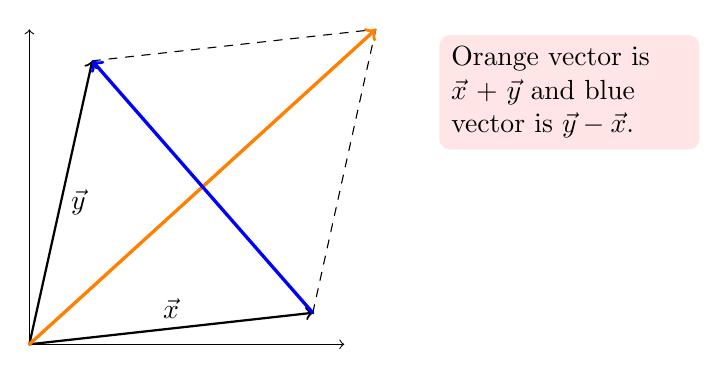
\begin{tikzpicture}
			[scale=4,line cap=round,
			%Styles
			axes/.style=,
			important line/.style={very thick},
			information text/.style={rounded corners,fill=red!10,inner sep=1ex},
			dot/.style={circle,inner sep=1pt,fill,label={#1},name=#1}			
			]
			
			%Colors
			\colorlet{anglecolor}{green!50!black}	%angle arcs/lines
			
			%The graphic
			\begin{scope}[axes]
				\draw[->] (0,0) -- (0,1);
				\draw[->] (0,0) -- (1,0);
			\end{scope}
			
			\draw[->,thick] (0,0) -- node[above] {$\vec{x}$} (.9, .1);
			\draw[->,thick] (0,0) -- node[right] {$\vec{y}$} (.2, .9);
			
			\draw[dashed] (.9,.1) -- (1.1,1);
			\draw[dashed] (.2,.9) -- (1.1,1);
			
			\path[name path=rleg] (.9,.1) -- (1.1,1);
			\path[name path=tleg] (.2,.9) -- (1.1,1);
			
			\draw[->,very thick,orange] (0,0) -- (1.1,1);
			\draw[->,very thick,blue] (.9,.1) -- (.2,.9);
			
			\draw[xshift=1.3cm](0,.8)
				node[right,text width=3cm,information text]
				{
					Orange vector is $\vec{x} + \vec{y}$ and blue vector is $\vec{y} - \vec{x}$.
				};
		\end{tikzpicture}
		\end{center}
		
\section{Points}
	$\mathbb{R}^2 \text{ and } \mathbb{R}^3$ can be used to define points on a plane and in space, respectively.
	\begin{center}
	\begin{tikzpicture}
		[scale=2,line cap=round,
		%Styles
		axes/.style=,
		important line/.style={very thick},
		information text/.style={rounded corners,fill=red!10,inner sep=1ex},
		dot/.style={circle,inner sep=1pt,fill,label={#1},name=#1}			
		]
		
		%Colors
		\colorlet{anglecolor}{green!50!black}	%angle arcs/lines
		
		%The graphic
		%\draw[help lines,step=0.5cm,loosely dashed] (-.4,-.4) grid (1.4,1.4);
		
		\begin{scope}[axes]
			\draw[->] (-.2,0) -- (1.5,0) node[right] {$x$} coordinate(x axis);
			\draw[->] (0,-.2) -- (0,1.5) node[above] {$y$} coordinate(y axis);
		\end{scope}
		
		\draw[->,thick,orange] (0,0) -- node[left=3pt] {$\vec{r}$} (1.2,1.2);
		\node [dot=P] at (1,1) {};
		\filldraw[fill=green!20,draw=anglecolor] (0,0) -- node[right=3pt,above,black] {$\theta$}(3mm,0pt) arc (0:45:3mm);
		
		\draw[xshift=1.8cm] (0,.8)
			node[right,text width=5cm,information text]
			{
				\begin{IEEEeqnarray}{rCl}
					\vec{OP} & = & (x_1, x_2)\\
					r & = & \sqrt{x_1^2 + x_2^2}\\
					x_1 & = & r\cos\theta\\
					x_2 & = & r\sin\theta
				\end{IEEEeqnarray}
			};
		
	\end{tikzpicture}
	
	\begin{tikzpicture}
		[scale=3,line cap=round,
		%Styles
		axes/.style=,
		important line/.style={very thick},
		information text/.style={rounded corners,fill=red!10,inner sep=1ex},
		dot/.style={circle,inner sep=1pt,fill,label={#1},name=#1}			
		]
		
		%Colors
		\colorlet{anglecolor}{green!50!black}	%angle arcs/lines
		
		%The graphic
		\begin{scope}[axes]
			\draw[<-] (-.5,-.5) node[right,below] {$x$} coordinate(x axis) -- (0,0);
			\draw[->] (0,0) -- (.7,0) node[right,below] {$y$} coordinate(y axis);
			\draw[->] (0,0) -- (0,.7) node[right,above] {$z$} coordinate(z axis);
		\end{scope}
		
		\draw[->,thick,orange] (0,0) -- node[above=3pt] {$\vec{r}$} (.6,.4);
		\node [dot=P] at (.6,.4) {};
		
		\filldraw[fill=green!20,draw=anglecolor] (0,0) -- (1.5mm,1mm) arc (15:120:1mm) node[above=5pt,right=2pt,black,font=\small] {$\phi$};
		
		\path [name path=zint] (-.25,-.25) -- (1,-.25);
		\path [name path=dropdown] (.6,.4) -- (.6, -1);
		\draw [name intersections={of=zint and dropdown, by=t}]
			[dashed] (.6,.4) -- (t);
		\draw [dashed] (-.25,-.25) -- (t);
		\draw[->] (0,0) -- (t);
		
		\path [name path=oq] (0,0) -- (t);
		\path [name path=phicircle] (0,0) circle (1mm);
		
		\filldraw [name intersections={of=oq and phicircle, by=u}]
			[fill=green!20,draw=anglecolor] (0,0) -- (u) arc (-20:-135:1mm) node[right=3pt,below,black,font=\small] {$\theta$};
			
		\draw[xshift=1cm]
			node[right,text width=6.5cm,information text]
			{
				The \textbf{spherical coordinates} (Figure \ref{fig:spherical}) defined by $(r,\phi,\theta)$, where $\theta$ is \textit{azimuth} along the equator and $\phi$ is \textit{inclination} from the meridian, can be converted to Cartesian coordinates.
				\begin{IEEEeqnarray}{rCl}
					r & = & \sqrt{x_1^2+x_2^2+x_3^2}\\
					x_1 & = & r\sin\phi\cos\theta\\
					x_2 & = & r\sin\phi\sin\theta\\
					x_3 & = & r\cos\theta
				\end{IEEEeqnarray}
			};
	
	\end{tikzpicture}
	\end{center}		
	
	\begin{figure}[htb]
		\centering
		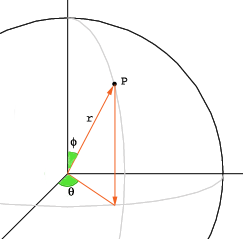
\includegraphics[width=0.4\textwidth]{vectorsfig3.png}
		\caption{Spherical coordinates.}
		\label{fig:spherical}
	\end{figure}
	
\section{Lines}
	There are two ways to specify a line with vectors: either as passing through a point in a direction, or as passing through 2 points.
	
	With the former method, given a nonzero vector $\vec{u}$, the line through the origin in the direction of $\vec{u}$ consists of all points whose position vectors are multiples of $\vec{u}$. If we translate all points by a vector $\vec{v}$, we get a generic definition for a line.
	\begin{equation}
		l = t\vec{u} + \vec{v} \quad \forall \ t \in \mathbb{R} \text{ and } \vec{u}\neq 0
	\end{equation}
	
	This is called the \textbf{parametric representation} of a line where $t$ is the \textbf{parameter}.
	
	When given two position vectors $\vec{a} \text{ and } \vec{b}$, it is possible to represent the line passing through both as such:
	
	\begin{IEEEeqnarray}{rCl}
		\vec{x} & = & t(\vec{b}-\vec{a}) + \vec{a}\\
		\vec{x} & = & (1-t)\vec{a} + t\vec{b}
	\end{IEEEeqnarray}
	
	When $t=0, \vec{x} = \vec{a}$ and when $t=1, \vec{x} = \vec{b}$.
	
\section{Planes}
	There is a unique plane that will contain any two nonzero vectors. The parametric representation of a plane is as follows:
	\begin{equation}
		\mathbf{x} = \vec{x_0} + s\vec{u} + t\vec{v}
	\end{equation}
	
	$\vec{x_0}$ is the linear shift of the origin. Note that if $\vec{x_0} = 0$, the plane is a linear combination of the vectors $\vec{u}$ and $\vec{v}$. Another condition for the plane is that $\vec{u}$ and $\vec{v}$ must be \textbf{linearly independent}, meaning neither is a scalar multiple of the other.
	
	A characteristic property of planes is that if the points $\mathbf{p}$ and $\mathbf{q}$ are both in the plane, the line that passes through them is entirely in the plane as well.
	
%		\def\enotesize{\normalsize}
%		\theendnotes
\end{document}